
We first summarize the economic layer of the incentivization scheme. At this
level, we assume the existence of an ideally secure and efficient payment layer
and proceed to outline the high-level policy design. The challenge here is to
engineer the flow of money in a way that is both economically stable yet still
adheres to the core mission of the Tor Project.

\subsection{Economic Policy}
The moneTor scheme allows for relays to offer a \emph{premium bandwidth} product
to Tor users in exchange for monetary payments. Under this framework,
financially willing users send payments directly to each relay along their circuits
in exchange for higher internet bandwidth and faster download speeds relative to
unpaid users. % The moneTor tokens themselves can be viewed as wrappers for some
% external financial asset that is converted at an exchange service.
The moneTor tokens %assets
may be any form of programmatic money which satisfies the standard properties of
\textit{scarcity}, \textit{fungibility}, \textit{divisibility},
\textit{durability}, and
\textit{transferability}~\cite[p.3]{crump2011phenomenon} A schematic of the cash
flow cycle is illustrated in Figure~\ref{fig:economic}.
\begin{figure}[h] \centering
  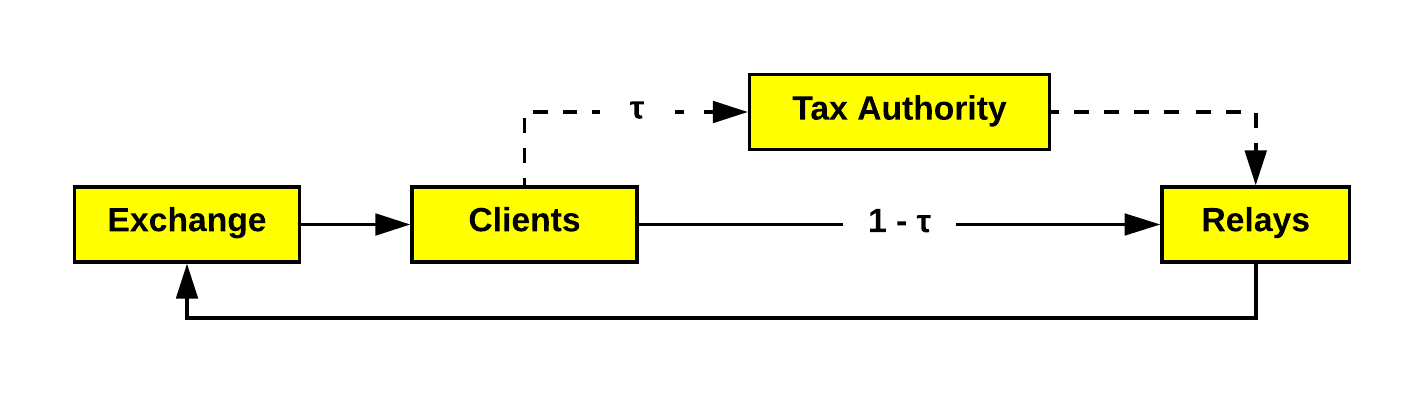
\includegraphics[trim={0.5cm, 0.5cm, 0.5cm, 0.5cm}, clip, scale=0.7]{images/economic_diagram.png}
  \caption[Cash Flow]{Cash Flow --- movement of moneTor tokens through the
    network. The value $\tau$ denotes the fraction of money that is collected
    for taxation purposes.}
  \label{fig:economic}
\end{figure}
We introduce a novel concept within the field in the form of a
taxation element. Intuitively, the shape of the network that will
emerge in a purely profit-seeking environment may not perfectly
correspond with the central goals of the Tor Project. The Tor Project
may for instance desire to compensate certain types of relays more
than others in order to improve the overall quality of the network
(e.g., supporting areas where anonymity is particularly important but
financial resources scarce). To this end, we accommodate for a stream
of taxed income that is anonymously diverted into a shared pool of
funds. These funds are selectively redistributed to relays via a
transparent policy.  In essence, taxation provides a tunable control
mechanism for The Tor Project to shape the topology of the network
towards some notion of optimal diversity and performance. The exact
content of such policy is an active subject of research that is
orthogonal to our paper. \op{Cite 2 or 3 papers that disagree on the
  best notion of diversity.}

A key economic question to address is the issue of price determination. While it
would be tempting to enlist some market-based mechanisms to set premium
bandwidth prices, any price differentiation between clients or relays inevitably
leaks more information. This leakage becomes more severe with higher granularity
payment options as adversaries begin to use price to link payment channels and
circuits. We therefore impose the constraint that all users should pay a single
uniform price for premium bandwidth at any time $t$. This price may be set
through a centralized calculation by the authorities or a more dynamical
consensus vote reached by the network.

\subsection{Incentivized Conformity} In a decentralized network, there is no
practical way to enforce standard behavior at each local node. We must therefore
consider whether all nodes are rationally incentivized to obey the stipulated
policies. For instance, we cannot guarantee that relays will actually confer
premium bandwidth to paying users. Even though the relay has no particular
reason to deviate, the client should periodically monitor her bandwidth and only
make payments when they appear to be making a difference. The relationship
between the client and relay can then be modeled as a game theoretic tit-for-tat
dynamic.

At the opposite end of the spectrum, relays might overly prioritize premium
circuits while rejecting all traffic from unpaid users. They might also attempt
to game the tax redistribution process to gain larger share of the proceeds. The
bandwidth measurement authorities must anticipate such modes of deviation from
the standard behavior to ensure that the risk for a relay to get blacklisted
from the network is greater than the incremental gains it might attain from
cheating. These attacks, while manageable, suggest that it would be prudent to
limit the complexity of our economic policies until we can better study
behavioral deviation dynamics in the live network.

%%% Local Variables:
%%% mode: latex
%%% TeX-master: "../main"
%%% End:
